\documentclass[11pt,aspectratio=169]{beamer}

\usepackage[T1]{fontenc} % pour le français
\usepackage[utf8]{inputenc}
\usepackage{lmodern}
\usepackage[french]{babel}
\usepackage{graphicx}
\usepackage{hyperref}
\usepackage{xcolor}
\usepackage{amsmath}
\usepackage{csquotes}
\usepackage{caption} 
\usepackage{subcaption} % for subfigures
% \captionsetup[figure]{font={small, sf},labelformat=empty}
\usepackage{amsfonts}
\usepackage{listings}
\usepackage[natbib=true,style=authortitle,backend=bibtex,useprefix=true]{biblatex}

% Links to other files
\addbibresource{references.bib}
\graphicspath{{figures/}}


% Beamer template customisation
\beamertemplatenavigationsymbolsempty
\setbeamertemplate{page number in head/foot}[totalframenumber] % numéros de slides
\setbeamercovered{transparent}
\usetheme{Madrid}
\usecolortheme{default}

% Setup colors title page + footline
% \definecolor{deepblue}{RGB}{0, 50, 100} 
\definecolor{deepblue}{RGB}{183, 110, 121} 
\setbeamercolor{title}{bg=deepblue, fg=white} 
\setbeamercolor{frametitle}{bg=deepblue, fg=white}
\setbeamercolor{footline}{bg=deepblue, fg=white}
\setbeamercolor{author in head/foot}{bg=deepblue, fg=white} 
\setbeamercolor{title in head/foot}{bg=deepblue, fg=white} 
\setbeamercolor{date in head/foot}{bg=deepblue, fg=white}

% No more bold font in footline
\setbeamerfont{author in head/foot}{series=\normalfont}
\setbeamerfont{title in head/foot}{series=\normalfont}
\setbeamerfont{date in head/foot}{series=\normalfont} 
\setbeamerfont{footline}{series=\normalfont} 

% TITLEPAGE
\author[Gendron \& Guibon]{\large Barbara Gendron-Audebert$^{1,2}$ et Gaël Guibon$^1$ \\ \texttt{\{prénom.nom\}@loria.fr}}
\title[\textsl{SentEmoContext} (SEC) : ERC en contexte]{SEC : contexte émotionnel phrastique intégré pour la reconnaissance émotionnelle efficiente dans la conversation \vspace{5pt}}
% \subtitle{\vspace{10pt} Session commune 1 - JEP-TALN 2024}
\date[JEP-TALN 2024 - 9 juillet 2024]{JEP-TALN 2024, 09 juillet 2024, Toulouse}
\institute[LORIA, UL, CNRS]{\small(1) LORIA, Université de Lorraine, CNRS \qquad (2) Université du Luxembourg}

\begin{document}

\begin{frame}[plain]
\vspace*{5pt}
	\begin{figure} 
	\hspace*{0.5cm}
	\begin{minipage}[c]{.42\linewidth} 
	\includegraphics[scale=0.04]{unilu.png} 
	\end{minipage} \hfill 
	\begin{minipage}[c]{.53\linewidth} 
	\includegraphics[scale=0.25]{labo-logos.pdf} 
	\end{minipage} 
	\end{figure}
	\vspace*{10pt}
	\titlepage
	
\end{frame}

\section{Introduction}

\begin{frame}{Contexte}
    Motivations
\end{frame}

\begin{frame}{Objectifs}
    
    Objectif global :
    \begin{itemize}
        \item Détection et identification des émotions dans le contenu généré par les utilisateurs
    \end{itemize}
    \vspace{10pt}
    Cadre de l'étude : % Pour réaliser ces objectifs "grandes directions" on a posé un cadre d'étude qui permet de vérifier nos hypothèses
    \begin{itemize}
        \item Dialogues sous forme de conversations dyadiques % le type de données que l'on étudie
        \item Reconnaissance d'Émotions en Conversation (ERC) % la tâche que l'on va chercher à évaluer 
    \end{itemize}
    \vspace{10pt}
    Questions de recherche :
    \begin{itemize}
        \item Comment utiliser l'information provenant du contexte conversationnel pour guider la détection d'émotions en conversation ?
        \item Est-ce que la prise en compte du contexte conversationnel permet d'améliorer la détection d'émotions en conversation dans le cas dyadique ?
    \end{itemize}
\end{frame}

\section{État-de-l'art}

\begin{frame}{Travaux connexes}
    
\end{frame}

\begin{frame}{Apport du \textsl{deep learning}}
    \begin{itemize}
        \item La profondeur du réseau neuronal permet de ... la subtilité du discours
        \item De nombreuses structures séquentielles à disposition
        \item Les modèles neuronaux obtiennent des résultats état-de-l'art en ERC~\footfullcite{Poria:2019}$^{,}$\footfullcite{Pereira:2022}
    \end{itemize}
\end{frame}

\begin{frame}{Apport du \textsl{metric learning}}

\end{frame}

\begin{frame}{Réseaux siamois}
Architecture présentée dans le papier original~\footfullcite{Koch:2015}
    \only<1>{
        \begin{figure}
            \centering
            \includegraphics[width=0.45\textwidth]{koch1.png}
        \end{figure}
    }
    \only<2>{
        \begin{figure}
            \centering
            \includegraphics[width=0.45\textwidth]{koch2.png}
        \end{figure}
    }
    \only<3>{
        \begin{figure}
            \centering
            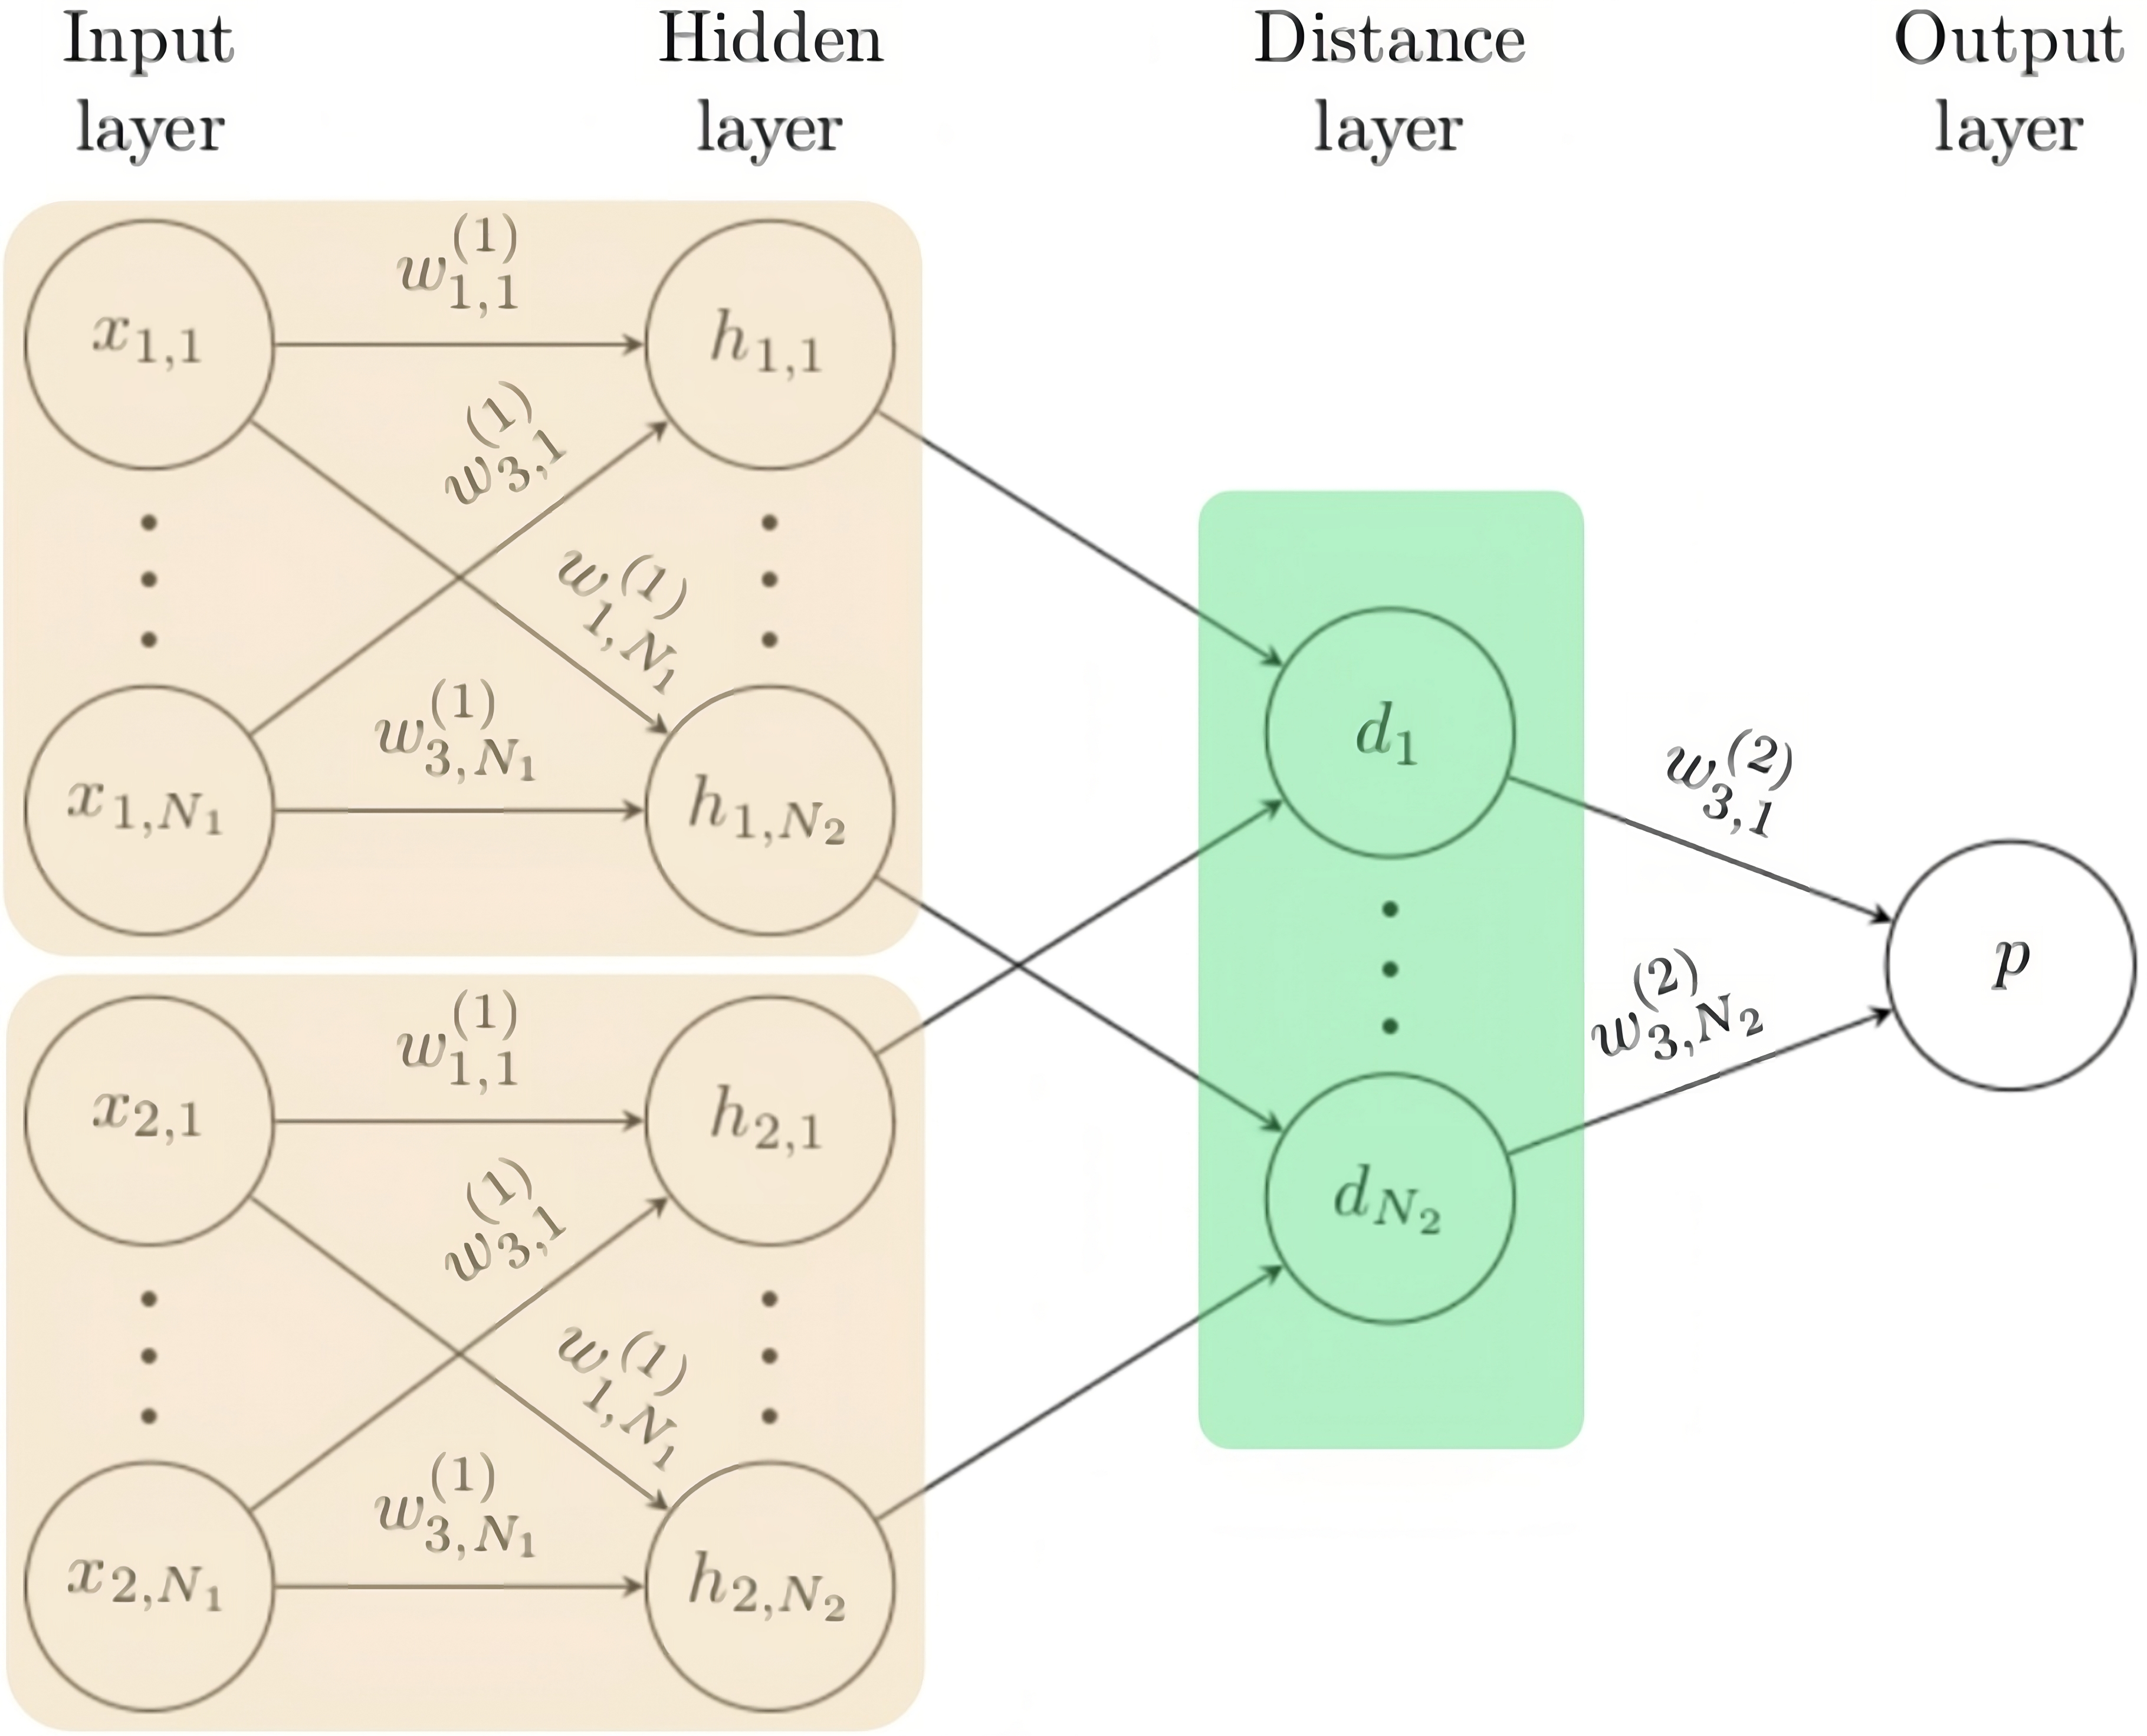
\includegraphics[width=0.45\textwidth]{koch3.png}
        \end{figure}
    }
\end{frame}

\begin{frame}{\textsl{Triplet loss} : fonction de coût par triplets}

\begin{equation*}
    \mathcal{L}(a, p, n) = \text{max}\left\{ d(a, p) - d(a, n) + \texttt{marge}, 0\right\}
\end{equation*}

\only<1>{
    \begin{figure}
        \centering
        \includegraphics[width=0.6\textwidth]{triplet_loss_no_margin.png}
    \end{figure}
}
\only<2>{
    \begin{figure}
        \centering
        \includegraphics[width=0.6\textwidth]{triplet_loss_margin.png}
    \end{figure}
}
\end{frame}

\section{Méthodologie}

\begin{frame}{Protocole expérimental}
    Jeu de données \texttt{DailyDialog}~\footfullcite{Li:2017}
    \begin{itemize}
        \item 13 118 dialogues dyadiques en anglais sur des sujets de la vie quotidienne
        \item<2-> Annotation au niveau du tour de parole : \texttt{happiness}, \texttt{anger}, \texttt{disgust}, \texttt{fear}, \texttt{surprise}, \texttt{sadness} et \texttt{no emotion}
    \end{itemize}

\visible<3->{
    \begin{figure}[h]
        \centering
        % \caption{\centering Description des données de \texttt{DailyDialog}}
        \begin{subfigure}[t]{0.45\textwidth}
            \centering
            \includegraphics[width=\textwidth]{topic-distib.png}
            \caption{\centering Répartition des sujets des dialogues}
            \label{fig:topics}
        \end{subfigure}
        \hfill
        \begin{subfigure}[t]{0.45\textwidth}
            \centering
            \includegraphics[width=\textwidth]{train-pretty.png}
            \caption{\centering Distribution des émotions dans les données d'entraînement}
            \label{fig:emotions}
        \end{subfigure}
        \label{fig:dd-desc}
    \end{figure}
}
\end{frame}

\begin{frame}{Évaluations quantitative et qualitative}
    \framesubtitle{Métriques d'évaluation}
    
\end{frame}

\begin{frame}{Évaluations quantitative et qualitative}
    \framesubtitle{Le MCC : \textsl{Matthews Correlation Coefficient}}
    
\end{frame}

\begin{frame}{Évaluations quantitative et qualitative}
    \framesubtitle{Subjectivité de l'annotation}
    
\end{frame}

\section{Résultats}

\begin{frame}{Résultats quantitatifs}
    
\end{frame}

\begin{frame}{Évaluation qualitative}
    
\end{frame}

\section{Conclusion}

\begin{frame}{Reconnaissance d'émotions en contexte}
    
\end{frame}

\begin{frame}{Limitations}
    
\end{frame}

\begin{frame}{Perspectives}
    Aller vers la détection plus subtile, d'émotions plus subtiles et pourquoi pas lien avec ironie ?
\end{frame}


\begin{frame}[plain]
    \begin{center}
        {\color{deepblue}\Huge Merci pour votre attention !}
        
        \vspace{0.5cm}
        
        \begin{figure}[h]
            \centering
            \begin{minipage}{0.45\textwidth}
                \centering
                \includegraphics[width=0.8\textwidth]{qrcode.jpg}
                \caption{Site personnel}
            \end{minipage}
            \hspace{0.05\textwidth}
            \begin{minipage}{0.45\textwidth}
                \centering
                \includegraphics[width=0.8\textwidth]{qrcode.jpg}
                \caption{Code SentEmoContext}
            \end{minipage}
        \end{figure}
    \end{center}
\end{frame}

\section{Bibliographie}

\begin{frame}[t,allowframebreaks]
\frametitle{Références}
\printbibliography
\end{frame}

\end{document}
